\chapter{A cellular quotient}

In this chapter, we construct a diagrammic representation of a quotient of $\TL(D_n)$ that will be used to show that this particular quotient is cellular.

\section{Pair-free Temperley-Lieb algebra}\label{sec:pairfree}

We will define the \emph{pair-free Temperley--Lieb algebra of type $D_{n}$}, denoted $\PFTL(D_{n})$, to be the quotient of $\TL(D_n)$ with the additional relation $b_1b_{\overline{1}}=0$. 
Since the monomial basis forms a basis for $\TL(D_n)$ and the relation $b_1b_{\overline{1}}=0$ eliminates the monomials indexed by the type I heaps but has no impact on the monomials indexed by the type II heaps, the following proposition holds.

\begin{proposition}
Let $\b_w$ be the image of $b_w$ in the quotient $\PFTL(D_n)$. Then \\ $\{\b_w: H(w)\text{ is of type II}\}$ is a basis for $\PFTL(D_n)$.
\qed
\end{proposition}


Note that if $w\in\FC(D_n)$ and no reduced expression of $w$ has $s_{\overline{1}}s_1$ as a subword, the heap of $w$ is of type II. In this case, we can safely identify $\b_w$ with $b_w$. We can represent $\PFTL(D_{n})$ in terms of generators and relations in a similar fashion to that of $\TL(D_n)$.

\begin{remark}\label{def:pfTL(D)}
The algebra $\PFTL(D_{n})$ ($n\ge4$)  is the unital $\Z[\delta]$-algebra generated by $\b_{\overline{1}},\b_{1},\b_{2},\ldots,\b_{n-1}$ with defining relations
\begin{enumerate}[leftmargin=0.6in]
\item $\b_{i}^{2}=\delta \b_{i}$ for all $i$, where $\delta$ is an indeterminate;
\item $\b_{i}\b_{j} = \b_{j}\b_{i}$ if $s_i$ and $s_j$ are not connected in the Coxeter graph of type $D_n$;
\item $\b_{i}\b_{j}\b_{i} = \b_{i}$ if $s_i$ and $s_j$ are connected in the Coxeter graph of type $D_n$;
\item $\b_{1}\b_{\overline{1}}=0.$
\end{enumerate}
\end{remark}

%In order to construct a diagrammatic representation of $\PFTL(D_n)$, we need to first define simple representations.
%%%%%%%%%simple representations %%%%%%%%%%%%%%%%%%%%%%%%
%\section{Simple representations}



%\begin{example}\label{vertequiv}
%Let $\w_1$ be the same reduced expression as in Example~\ref{simplerep}. By applying the commutation $s_1s_3=s_3s_1$, we obtain the reduced expression $\w_2=s_{\overline{1}}s_3s_2s_3s_1$. Since the concrete simple representation of $\w_2$ shown in Figure~\ref{vertclass} is the same diagram as the concrete simple representation of  $\w_1$, then $\w_1$ and $\w_2$ are vertically equivalent. Then applying the long braid relation $s_3s_2s_3=s_2s_3s_2$ to $\w_2$ we obtain a third reduced expression $\w_3=s_{\overline{1}}s_2s_3s_2s_1$ with concrete representation given in Figure~\ref{notvertclass}. The concrete representation of $d_{\w_3}$  is thus not vertically equivalent of neither $\w_1$ nor $\w_2$.
%\end{example}
%
%\begin{figure}[h]
%\centering
%\begin{subfigure}[b]{0.45\textwidth}
%\centering
%\begin{tikzpicture}[scale=1]
%\topbox{2};
%\draw (1,2) arc (-180:0:0.5 and 0.4);
%\draw[fill=cyan, draw=white]{(1.5,1.6) circle (2.8pt)};
%\draw (1,0) arc (180:0:0.5 and 0.4);
%\draw[fill=cyan, draw=white]{(1.5,0.4) circle (2.8pt)};
%\draw (3,2) arc (-180:0:0.5 and 0.4);
%\draw (5,2) -- (5,0);
%\draw[dashed] (1.5,1.5) -- (1.5,0.5);
%\draw[dashed] (3.5,1.5) -- (3.5,0.5);
%\middlebox{0};
%\draw (1,0)  -- (1,-2);
%\draw (3,0)  arc (180:0:0.5 and 0.4) ;
%\draw (2,0)  arc(-180:0:0.5 and 0.4);
%\draw (2,-2)  arc(180:0:0.5 and 0.4);
%\draw (4,0) -- (4,-2);
%\draw (5,0) -- (5,-2);
%\draw[dashed] (2.5,-0.5) -- (2.5,-1.5);
%\bottombox{-2};
%\draw (3,-2)  arc (-180:0:0.5 and 0.4) ;
%\draw (3,-4)  arc (180:0:0.5 and 0.4) ;
%\draw (1,-2)  arc (-180:0:0.5 and 0.4) ;
%\draw (1,-4)  arc (180:0:0.5 and 0.4) ;
%\draw (5,-2) -- (5,-4);
%\draw[dashed] (1.5,-2.5) -- (1.5,-3.5);
%\draw[dashed] (3.5,-2.5) -- (3.5,-3.5);
%\end{tikzpicture}
%\caption{Representations of $d_{\w_1}$ and $d_{\w_2}$.}
%\label{vertclass}
%\end{subfigure}
%\begin{subfigure}[b]{0.45\textwidth}
%\centering
%\begin{tikzpicture}[scale=0.7]
%\topbox{2};
%\draw (1,2) arc (-180:0:0.5 and 0.4);
%\draw[fill=cyan, draw=white]{(1.5,1.6) circle (2.8pt)};
%\draw (1,0) arc (180:0:0.5 and 0.4);
%\draw[fill=cyan, draw=white]{(1.5,0.4) circle (2.8pt)};
%\draw (3,2) -- (3,0);
%\draw (4,2) -- (4,0);
%\draw (5,2) -- (5,0);
%\draw[dashed] (1.5,1.5) -- (1.5,0.5);
%\middlebox{0};
%\draw (1,0)  -- (1,-2);
%\draw (2,0)  arc (-180:0:0.5 and 0.4) ;
%\draw (2,-2)  arc (180:0:0.5 and 0.4) ;
%\draw (4,-2)  -- (4,0);
%\draw (5,0) -- (5,-2);
%\draw[dashed] (2.5,-1.5) -- (2.5,-0.5);
%\middlebox{-2};
%\draw (1,-2)  -- (1,-4);
%\draw (3,-2)  arc (-180:0:0.5 and 0.4) ;
%\draw (3,-4)  arc (180:0:0.5 and 0.4) ;
%\draw (2,-4)  -- (2,-2);
%\draw (5,-4) -- (5,-2);
%\draw[dashed] (3.5,-2.5) -- (3.5,-3.5);
%\middlebox{-4};
%\draw (1,-6)  -- (1,-4);
%\draw (2,-4)  arc (-180:0:0.5 and 0.4) ;
%\draw (2,-6)  arc (180:0:0.5 and 0.4) ;
%\draw (4,-4)  -- (4,-6);
%\draw (5,-4) -- (5,-6);
%\draw[dashed] (2.5,-4.5) -- (2.5,-5.5);
%\bottombox{-6};
%\draw (3,-6)  -- (3,-8);
%\draw (1,-6)  arc (-180:0:0.5 and 0.4) ;
%\draw (1,-8)  arc (180:0:0.5 and 0.4) ;
%\draw (4,-6)  -- (4,-8);
%\draw (5,-6) -- (5,-8);
%\draw[dashed] (1.5,-6.5) -- (1.5,-7.5);
%\end{tikzpicture}\caption{Representation of $d_{\w_2}$}
%\label{notvertclass}
%\end{subfigure}
%\caption{Two concrete simple representations for a non-fully commutative element in $W(D_4)$.}\label{simplerep}
%\end{figure} 


%%%%%%%%%%%%% admissible diagrams type 2 %%%%%%%%%%%%%

\begin{section}{Loop-free diagram algebra}\label{sec:loopfree}
We will now construct a diagram algebra that turns out to be a diagrammatic representation of $\PFTL(D_n)$.
\begin{definition}\label{def:D_nII}
\rm Let $\LFD(D_{n})$ be the $\Z[\delta]$-algebra equal to the quotient of $\DTL(D_n)$ with the additional relation given in Figure~\ref{decloop}.
\end{definition}

\begin{figure}[!ht]
\centering
\begin{align*}
\begin{tabular}[c]{l}
\begin{tikzpicture}
\dlp{0}{-1};
\end{tikzpicture}
\end{tabular}
&=~0
\end{align*}
\caption{Additional defining relation of $\LFD(D_n)$.}
\label{decloop}
\end{figure}


 Let $\d_w$ denote the image of $d_w$ in the quotient. Since the relation in Figure~\ref{decloop} has no effect on the type II diagrams, we can safely identify $\d_{w}$ with $d_{w}$ when $d_w$ is of type II and will use the same diagram to represent $\d_w$. Since $d_{\overline{1}},d_1,\ldots,d_n$ generate the type I and type II diagrams and each $d_i$ is a type II diagram, it follows that $\LFD(D_n)$ is generated by $\d_{\overline{1}},\d_1,\d_2,\ldots,\d_{n-1}$.

\begin{proposition}\label{rem:DII relations hold}
\rm Each of the following relations are satisfied for $\LFD(D_{n})$.
\begin{enumerate}[leftmargin=0.6in]
\item $\d_{i}^{2}=\delta \d_{i}$ for all $i$;
\item $\d_{i}\d_{j}=\d_{j}\d_{i}$ if $s_i$ and $s_j$ are not connected in the Coxeter graph of type $D_n$;
\item $\d_{i}\d_{j}\d_{i}=\d_{i}$ if $s_i$ and $s_j$ are connected in the Coxeter graph of type $D_n$;
\item $\d_{1}\d_{\overline{1}}=0.$
\end{enumerate}
\end{proposition}
\begin{proof}
Since the first three relations hold in $\TL(D_n)$, the only relation left to check is $\d_{1}\d_{\overline{1}}=0$. We see that

\begin{align*}
\d_1\d_{\overline{1}} &=
\begin{tabular}[c]{l}
\begin{tikzpicture}[scale=1]
\sixbox{0};
\draw (1,0) arc (-180:0:0.5 and 0.4);
\draw (1,-2) arc (180:0:0.5 and 0.4);
\draw (3,0) -- (3,-2);
\draw (4,0) -- (4,-2);
\draw (5,0) -- (5,-2);
\draw (6,0) -- (6,-2);
\node at (5.5,-1) {$\cdots$};
\sixbox{-2};
\draw (1,-4) arc (180:0:0.5 and 0.4);
\draw (1,-2) arc (-180:0:0.5 and 0.4);
\draw (3,-4) -- (3,-2);
\draw (4,-4) -- (4,-2);
\draw (5,-4) -- (5,-2);
\draw (6,-4) -- (6,-2);
\node at (5.5,-3) {$\cdots$};
\draw[fill=cyan, draw=white]{(1.5,-2.4) circle (2.8pt)};
\draw[fill=cyan, draw=white]{(1.5,-3.6) circle (2.8pt)};
\end{tikzpicture}
\end{tabular}\\
&= 
\begin{tabular}[c]{l}
\begin{tikzpicture}[scale=1]
\sixbox{0};
\draw (1,0) arc (-180:0:0.5 and 0.4);
\draw (1,-2) arc (180:0:0.5 and 0.4);
\draw (3,0) -- (3,-2);
\draw (4,0) -- (4,-2);
\draw (5,0) -- (5,-2);
\draw (6,0) -- (6,-2);
\node at (5.5,-1) {$\cdots$};
\dlp{1.5}{-1};
\end{tikzpicture}
\end{tabular}\\
&=0.
\end{align*}
\end{proof}

%\begin{definition}\label{homo}
%Define $\phi: \PFTL(D_{n}) \to \LFD(D_{n})$ to be the $\Z[\delta]$-algebra homomorphism determined by $\phi(\b_{i})=\d_{i}$.  
%\end{definition}


The next proposition follows quickly from Proposition \ref{rem:DII relations hold} since $\LFD(D_{n})$ satisfies the relations given in Remark~\ref{def:pfTL(D)}.

\begin{proposition}\label{prop:surjective homo}
The map $\phi: \PFTL(D_{n}) \to \LFD(D_{n})$ determined by $\phi(\b_{i})=\d_{i}$ is a well-defined surjective $\Z[\delta]$-algebra homomorphism.
\textcolor{black}{\qed}
\end{proposition}

Since the $D$-admissible diagrams form a basis for $\DTL(D_{n})$ and the relation in (\ref{decloop}) eliminates the type I $D$-admissible diagrams but has no impact on the type II $D$-admissible diagrams, the following proposition holds.

\begin{proposition}
The images of the type II $D$-admissible diagrams form a basis for $\LFD(D_n)$. %and thus $\dim\left(\LFD(D_n)\right)=\frac{1}{2}{2n \choose n}$.
\qed
\end{proposition}

If $d$ is a $D$-admissible diagram, then we say that a non-propagating edge joining $i$ to $i+1$ (respectively, $i'$ to $(i+1)'$) is \emph{simple} if it is  identical to the edge joining $i$ to $i+1$ (respectively $i'$ to $(i+1)'$) in the simple diagram $d_i$. That is, an edge is simple if it joins adjacent vertices in the north face (respectively, south face) and is undecorated, except when one of the vertices is $1$ or $1'$, in which case it may be decorated by only a single decoration $\bcirc$.

Let $\w=s_{x_1}\cdots s_{x_k}$ be a reduced expression for $w\in\FC(D_n)$. Then $d=d_{x_1}\cdots d_{x_k}$. For each $d_{x_i}$, fix a concrete representation that has straight propagating edges and no unnecessary ``wiggling" of the simple non-propagating edges. Now, consider the concrete diagram that results from stacking the concrete simple diagrams $d_{x_1},\ldots,d_{x_k}$, rescaling vertically to recover the standard $k$-box, but not deforming any of the simple edges or applying any relations among the decorations. We will refer to this concrete diagram as the \emph{concrete simple representation of} $d_{\w}$. 

Since $w$ is fully commutative and vertical equivalence respects commutation, given two different reduced expressions $\w_1$ and $\w_2$ for $w$, the concrete simple representations $d_{\w_1}$ and $d_{\w_2}$ will be vertically equivalent (see Remark~\ref{vertequiv}). We define the vertical equivalence class of concrete simple representations to be the \emph{simple representation of }$d_w$. The simple representation of $d_w$ is designed to replicate the structure of the corresponding heap.

%We define $d_{\w_1}$ and $d_{\w_2}$ to be \emph{vertically equivalent} if we can deform non-simple edges of $d_{\w_1}$ to obtain $d_{\w_2}$.

\begin{example}\label{simplerep}
Let $\w=s_{\overline{1}}s_{3}s_{2}s_{1}$ be a reduced expression for $w\in\FC(D_4)$. The concrete simple representation of $d_{w}$ is shown in Figure~\ref{fig:simplerep} where the vertical dashed lines in the diagram indicate that the two non-propagating edges are part of the same generator.
\end{example}

\begin{figure}[!ht]
\centering
\begin{tabular}[c]{l}
\begin{tikzpicture}[scale=1]
\fivebox{2};
\draw (1,2) arc (-180:0:0.5 and 0.4);
\draw[fill=cyan, draw=white]{(1.5,1.6) circle (2.8pt)};
\draw (1,0) arc (180:0:0.5 and 0.4);
\draw[fill=cyan, draw=white]{(1.5,0.4) circle (2.8pt)};
\draw (3,2) -- (3,0);
\draw (4,2) -- (4,0);
\draw (5,2) -- (5,0);
\fivebox{0};
\draw (1,0)  -- (1,-2);
\draw (3,0)  arc (-180:0:0.5 and 0.4) ;
\draw (3,-2)  arc (180:0:0.5 and 0.4) ;
\draw (2,-2)  -- (2,0);
\draw (5,0) -- (5,-2);
\fivebox{-2};
\draw (1,-2)  -- (1,-4);
\draw (2,-2)  arc (-180:0:0.5 and 0.4) ;
\draw (2,-4)  arc (180:0:0.5 and 0.4) ;
\draw (4,-4)  -- (4,-2);
\draw (5,-4) -- (5,-2);
\fivebox{-4};
\draw (3,-6)  -- (3,-4);
\draw (1,-4)  arc (-180:0:0.5 and 0.4) ;
\draw (1,-6)  arc (180:0:0.5 and 0.4) ;
\draw (4,-4)  -- (4,-6);
\draw (5,-4) -- (5,-6);
\end{tikzpicture}
\end{tabular}
~$=$~
\begin{tabular}[c]{l}
\begin{tikzpicture}[scale=1]
\topbox{2};
\draw (1,2) arc (-180:0:0.5 and 0.4);
\draw[fill=cyan, draw=white]{(1.5,1.6) circle (2.8pt)};
\draw (1,0) arc (180:0:0.5 and 0.4);
\draw[fill=cyan, draw=white]{(1.5,0.4) circle (2.8pt)};
\draw (3,2) arc (-180:0:0.5 and 0.4);
\draw (5,2) -- (5,0);
\draw[dashed] (1.5,1.5) -- (1.5,0.5);
\draw[dashed] (3.5,1.5) -- (3.5,0.5);
\middlebox{0};
\draw (1,0)  -- (1,-2);
\draw (3,0)  arc (180:0:0.5 and 0.4) ;
\draw (2,0)  arc(-180:0:0.5 and 0.4);
\draw (2,-2)  arc(180:0:0.5 and 0.4);
\draw (4,0) -- (4,-2);
\draw (5,0) -- (5,-2);
\draw[dashed] (2.5,-0.5) -- (2.5,-1.5);
\bottombox{-2};
\draw (3,-2)  -- (3,-4);
\draw (4,-4)  -- (4,-2) ;
\draw (1,-2)  arc (-180:0:0.5 and 0.4) ;
\draw (1,-4)  arc (180:0:0.5 and 0.4) ;
\draw (5,-2) -- (5,-4);
\draw[dashed] (1.5,-2.5) -- (1.5,-3.5);
\end{tikzpicture}
\end{tabular}
\caption{Example of a simple representation.}\label{fig:simplerep}
\end{figure} 


%In order to show that $\phi$ is an isomorphisn, we need to first define simple representations.

 
\begin{lemma}\label{configs}
Let $\w$ be a reduced expression for $w\in \FC(D_n)$. Then the simple representation of $d_{\w}$ cannot have the configurations shown in Figure~\ref{notFC}.
\end{lemma}

\begin{figure}[!ht]
\begin{center}
 \begin{tikzpicture}[scale=1.1]
\tttbox{2};
%\draw (1,0)  -- (1,2);
\draw (1,2) arc (-180:0:0.5 and 0.4);
\draw (1,0) arc (180:0:0.5 and 0.4);
\draw[dashed] (1.5,1.5) -- (1.5,0.5);
\mmmidbox{0};
\draw (2,0)  arc(-180:0:0.5 and 0.4);
\draw (2,-2)  arc(180:0:0.5 and 0.4);
\draw (1,0) -- (1,-2);
\draw[dashed] (2.5,-0.5) -- (2.5,-1.5);
\bbbotbox{-2};
\draw (1,-2)  arc (-180:0:0.5 and 0.4) ;
\draw (1,-4)  arc (180:0:0.5 and 0.4) ;
%\draw (1,-2) -- (1,-4);
\draw[dashed] (1.5,-2.5) -- (1.5,-3.5);
\end{tikzpicture}
\quad\quad
 \begin{tikzpicture}[scale=1.1]
\tttbox{2};
%\draw (1,0)  -- (1,2);
\draw (2,2) arc (-180:0:0.5 and 0.4);
\draw (2,0) arc (180:0:0.5 and 0.4);
\draw[dashed] (2.5,1.5) -- (2.5,0.5);
\mmmidbox{0};
\draw (1,0)  arc(-180:0:0.5 and 0.4);
\draw (1,-2)  arc(180:0:0.5 and 0.4);
\draw (3,0) -- (3,-2);
\draw[dashed] (1.5,-0.5) -- (1.5,-1.5);
\bbbotbox{-2};
\draw (2,-2)  arc (-180:0:0.5 and 0.4) ;
\draw (2,-4)  arc (180:0:0.5 and 0.4) ;
%\draw (1,-2) -- (1,-4);
\draw[dashed] (2.5,-2.5) -- (2.5,-3.5);
\end{tikzpicture}
\end{center}
\caption{Impermissible configurations for a simple representation.}\label{notFC}
\end{figure}

%\quad
%\begin{tikzpicture}[scale=0.5]
%\ttlongbox{6};
%%\draw (1,0)  -- (1,2);
%\draw (7,6) arc (-180:0:0.5 and 0.4);
%\draw (7,4) arc (180:0:0.5 and 0.4);
%\draw[dashed] (7.5,4.5) -- (7.5,5.5);
%\mmidlongbox{4};
%\draw (6,4)  arc(-180:0:0.5 and 0.4);
%\draw (6,2)  arc(180:0:0.5 and 0.4);
%\draw (8,2) -- (8,4);
%\draw[dashed](6.5,2.5)--(6.5,3.5);
%\mmidlongbox{2};
%\draw (2,0)  arc(180:0:0.5 and 0.4);
%%\draw[dashed](2.5,0.5)--(2.5,1.5);
%\draw (7,0) -- (7,2);
%\draw (8,0) -- (8,2);
%\mmidlongbox{0};
%\draw (3,0) -- (3,-2);
%\draw (1,0)  arc(-180:0:0.5 and 0.4);
%\draw (1,-2)  arc(180:0:0.5 and 0.4);
%\draw[dashed](1.5,-0.5)--(1.5,-1.5);
%\draw (7,0) -- (7,-2);
%\draw (8,0) -- (8,-2);
%\node at (4.5,-1) {$\rightarrow$};
%%\draw (4,0)  arc(-180:0:0.5 and 0.4);
%%\draw (4,-2)  arc(180:0:0.5 and 0.4);
%%\draw[dashed](4.5,-0.5)--(4.5,-1.5);
%\mmidlongbox{-2};
%\draw (2,-2)  arc(-180:0:0.5 and 0.4);
%\draw (7,-2) -- (7,-4);
%\draw (8,-2) -- (8,-4);
%\mmidlongbox{-4};
%\draw (6,-4)  arc(-180:0:0.5 and 0.4);
%\draw (6,-6)  arc(180:0:0.5 and 0.4);
%\draw (8,-4) -- (8,-6);
%\draw[dashed] (6.5,-4.5) -- (6.5,-5.5);
%\bbotlongbox{-6};
%\draw (7,-6)  arc (-180:0:0.5 and 0.4) ;
%\draw (7,-8)  arc (180:0:0.5 and 0.4) ;
%%\draw (1,-2) -- (1,-4);
%\draw[dashed] (6.5,-6.5) -- (6.5,-7.5);
%\end{tikzpicture}

%\begin{figure}
%\begin{tabular}[c]{c}
% \begin{tikzpicture}[scale=0.8]
%\tbox{2};
%\draw (1,2) arc (-180:0:0.5 and 0.4);
%\draw[fill=cyan, draw=white]{(1.5,1.6) circle (2.8pt)};
%\draw (1,0) arc (180:0:0.5 and 0.4);
%\draw[fill=cyan, draw=white]{(1.5,0.4) circle (2.8pt)};
%\draw[dashed] (1.5,1.5) -- (1.5,0.5);
%\node[above,scale=0.8] at (1,2){$1$};
%\node[above,scale=0.8] at (2,2){$2$};
%\node[above,scale=0.8] at (3,2){$3$};
%\midbox{0};
%\draw (1,0)  -- (1,-2);
%\draw (2,0)  arc(-180:0:0.5 and 0.4);
%\draw (2,-2)  arc(180:0:0.5 and 0.4);
%\draw[dashed] (2.5,-0.5) -- (2.5,-1.5);
%\botbox{-2};
%\draw (1,-2)  arc (-180:0:0.5 and 0.4) ;
%\draw (1,-4)  arc (180:0:0.5 and 0.4) ;
%\draw[fill=cyan, draw=white]{(1.5,-2.4) circle (2.8pt)};
%\draw[fill=cyan, draw=white]{(1.5,-3.6) circle (2.8pt)};
%\draw[dashed] (1.5,-2.5) -- (1.5,-3.5);
%\end{tikzpicture}
%\end{tabular},
%\begin{tabular}[c]{c}
% \begin{tikzpicture}[scale=0.8]
%\tbox{2};
%\draw (1,0)  -- (1,2);
%\draw (2,2) arc (-180:0:0.5 and 0.4);
%\draw (2,0) arc (180:0:0.5 and 0.4);
%\draw[dashed] (2.5,1.5) -- (2.5,0.5);
%\midbox{0};
%\draw (1,0)  arc(-180:0:0.5 and 0.4);
%\draw (1,-2)  arc(180:0:0.5 and 0.4);
%%\draw (3,0) -- (3,-2);
%\draw[fill=cyan, draw=white]{(1.5,-0.4) circle (2.8pt)};
%\draw[fill=cyan, draw=white]{(1.5,-1.6) circle (2.8pt)};
%\draw[dashed] (1.5,-0.5) -- (1.5,-1.5);
%\botbox{-2};
%\draw (2,-2)  arc (-180:0:0.5 and 0.4) ;
%\draw (2,-4)  arc (180:0:0.5 and 0.4) ;
%\draw (1,-2) -- (1,-4);
%\draw[dashed] (2.5,-2.5) -- (2.5,-3.5);
%\end{tikzpicture}
%\end{tabular},
%\begin{tabular}[c]{c}
% \begin{tikzpicture}[scale=0.8]
%\ttbox{2};
%\draw (1,2) arc (-180:0:0.5 and 0.4);
%\draw (1,0) arc (180:0:0.5 and 0.4);
%\draw[dashed] (1.5,1.5) -- (1.5,0.5);
%\mmidbox{0};
%%\draw (1,0)  -- (1,-2);
%\draw (2,0)  arc(-180:0:0.5 and 0.4);
%\draw (2,-2)  arc(180:0:0.5 and 0.4);
%\draw[dashed] (2.5,-0.5) -- (2.5,-1.5);
%\bbotbox{-2};
%\draw (1,-2)  arc (-180:0:0.5 and 0.4) ;
%\draw (1,-4)  arc (180:0:0.5 and 0.4) ;
%\draw[dashed] (1.5,-2.5) -- (1.5,-3.5);
%\end{tikzpicture}
%\end{tabular},
%\begin{tabular}[c]{c}
% \begin{tikzpicture}[scale=1]
%\ttbox{2};
%%\draw (1,0)  -- (1,2);
%\draw (2,2) arc (-180:0:0.5 and 0.4);
%\draw (2,0) arc (180:0:0.5 and 0.4);
%\draw[dashed] (2.5,1.5) -- (2.5,0.5);
%\mmidbox{0};
%\draw (1,0)  arc(-180:0:0.5 and 0.4);
%\draw (1,-2)  arc(180:0:0.5 and 0.4);
%\draw (3,0) -- (3,-2);
%%\draw (3,0) -- (3,-2);
%\draw[dashed] (1.5,-0.5) -- (1.5,-1.5);
%\bbotbox{-2};
%\draw (2,-2)  arc (-180:0:0.5 and 0.4) ;
%\draw (2,-4)  arc (180:0:0.5 and 0.4) ;
%%\draw (1,-2) -- (1,-4);
%\draw[dashed] (2.5,-2.5) -- (2.5,-3.5);
%\end{tikzpicture}
%\end{tabular}
%\quad
%\begin{tabular}[c]{c}
%\begin{tikzpicture}[scale=0.6]
%\ttbox{4};
%%\draw (1,0)  -- (1,2);
%\draw (1,4) arc (-180:0:0.5 and 0.4);
%\draw (1,2) arc (180:0:0.5 and 0.4);
%\draw[dashed] (1.5,2.5) -- (1.5,3.5);
%\mmidbox{2};
%\draw (2,2)  arc(-180:0:0.5 and 0.4);
%\draw (2,0)  arc(180:0:0.5 and 0.4);
%\draw (1,0) -- (1,2);
%\draw[dashed](2.5,0.5)--(2.5,1.5);
%\mmidbox{0};
%\draw (2,0) -- (2,-2);
%\draw (1,0) -- (1,-2);
%\mmidbox{-2};
%\draw (2,-2)  arc(-180:0:0.5 and 0.4);
%\draw (2,-4)  arc(180:0:0.5 and 0.4);
%\draw (1,-2) -- (1,-4);
%\draw[dashed] (2.5,-2.5) -- (2.5,-3.5);
%\bbotbox{-4};
%\draw (1,-4)  arc (-180:0:0.5 and 0.4) ;
%\draw (1,-6)  arc (180:0:0.5 and 0.4) ;
%%\draw (1,-2) -- (1,-4);
%\draw[dashed] (1.5,-4.5) -- (1.5,-5.5);
%\end{tikzpicture}
%\end{tabular}
%\quad
%\begin{tabular}[c]{c}
% \begin{tikzpicture}[scale=0.8]
%\tttbox{2};
%\draw (1,2) arc (-180:0:0.5 and 0.4);
%\draw (1,0) arc (180:0:0.5 and 0.4);
%\draw[dashed] (1.5,1.5) -- (1.5,0.5);
%\draw (3,0) -- (3,2);
%\mmmidbox{0};
%%\draw (1,0)  -- (1,-2);
%\draw (2,0)  arc(-180:0:0.5 and 0.4);
%\draw (2,-2)  arc(180:0:0.5 and 0.4);
%\draw[dashed] (2.5,-0.5) -- (2.5,-1.5);
%\bbbotbox{-2};
%\draw (1,-2)  arc (-180:0:0.5 and 0.4) ;
%\draw (1,-4)  arc (180:0:0.5 and 0.4) ;
%\draw[dashed] (1.5,-2.5) -- (1.5,-3.5);
%\draw (3,-2) -- (3,-4);
%\end{tikzpicture}
%\end{tabular},
%
%where $i\in\{1,2,\ldots,n-4\}$.


\begin{proof}
Let $\w$ be a reduced expression for $w\in\FC(D_n)$. If $\w$ has either configuration in Figure~\ref{notFC}, then $\w$ has $s_{i+1}s_{i}s_{i+1}$ as a subword. Hence, $w$ is not fully commutative, which is a contradiction. 
\end{proof}

\begin{theorem}\label{index}
The type I and type II diagrams are indexed by the type I and type II heaps, respectively.
\end{theorem}

\begin{proof}
Let $\w=s_{x_{1}}\cdots s_{x_{n}}$ be a reduced expression for $w\in\FC(D_n)$. Consider the diagram $d_{w}=d_{x_{1}}\cdots d_{x_{n}}$. If $s_{1}s_{\overline{1}}$ is a subword of some reduced expression for $w$, then it is obvious that $d_{w}$  is a type I diagram. Now assume $d_{w}$ is a type I diagram. Clearly, $s_{\overline{1}}\in$ supp$(w)$ since $d_{\overline{1}}$ is the only simple diagram that contains decorations. It is also clear that $d_{w}$ contains only one loop, and hence, if $s_{1}s_{\overline{1}}$ is a subword of $\w$, then it only appears once. 
For $d_{w}$ to be a type I diagram, $d_{w}$ must contain one decorated loop. Consider the occurence of $s_{\overline{1}}$ involved in the loop. Without loss of generality, assume this occurence of $s_{\overline{1}}$ appears on the ``top" of the loop in the simple representation for $d_{\w}$. Since the configurations in Figure~\ref{notFC} cannot happen, there is no way for the loop edge to wander through the simple representation unless the portion of the diagram given in Figure~\ref{1bar1} appears in the simple representation $d(w)$.
\end{proof}

\begin{figure}[h]
\centering
 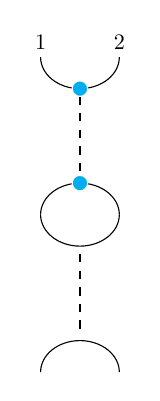
\begin{tikzpicture}[scale=1]
\tbox{2};
\draw (1,2) arc (-180:0:0.5 and 0.4);
\draw[fill=cyan, draw=white]{(1.5,1.6) circle (2.8pt)};
\draw (1,0) arc (180:0:0.5 and 0.4);
\draw[fill=cyan, draw=white]{(1.5,0.4) circle (2.8pt)};
\draw[dashed] (1.5,1.5) -- (1.5,0.5);
\node[above,scale=0.8] at (1,2){$1$};
\node[above,scale=0.8] at (2,2){$2$};
%\node[above,scale=0.8] at (3,2){$3$};
\botbox{0};
\draw (1,0)  arc (-180:0:0.5 and 0.4) ;
\draw (1,-2)  arc (180:0:0.5 and 0.4) ;
\draw[dashed] (1.5,-0.5) -- (1.5,-1.5);
\end{tikzpicture}
\caption{Portion of the simple representation from Theorem~\ref{index}.}
\label{1bar1}
\end{figure}

 %which corresponds to $s_{\overline{1}}s_1$. 

%There are two ways to produce a decorated loop. The first way is via $d_{\overline{1}}d_1$ which corresponds to $s_{\overline{1}}s_{1}$, in which case we are done. The other way requires the edge that forms the loop in the simple representation of $d_{\w}$ to change direction from right to left at some node. Since 

%is permissible since it corresponds to $s_{\overline{1}}s_2s_1$, then we must have
%\begin{center}
%\begin{tikzpicture}[scale=0.7]
%\ttlongbox{2};
%%\draw (1,0)  -- (1,2);
%\draw (1,2) arc (-180:0:0.5 and 0.4);
%\draw[fill=cyan, draw=white]{(1.5,1.6) circle (2.8pt)};
%\draw (1,0) arc (180:0:0.5 and 0.4);
%\draw[fill=cyan, draw=white]{(1.5,0.4) circle (2.8pt)};
%\draw[dashed] (1.5,1.5) -- (1.5,0.5);
%\mmidlongbox{0};
%%\draw (1,0)  -- (1,-2);
%\draw (2,0)  arc(-180:0:0.5 and 0.4);
%%\draw (2,-2)  arc(180:0:0.5 and 0.4);
%%\draw[dashed] (2.5,-0.5) -- (2.5,-1.5);
%\draw (8,0) -- (8,-2);
%\draw (6,0)  arc(-180:0:0.5 and 0.4);
%\draw (6,-2)  arc(180:0:0.5 and 0.4);
%\draw (7,0)  arc(180:0:0.5 and 0.4);
%\draw[dashed](6.5,-0.5)--(6.5,-1.5);
%\node at (4.5,-2){$\cdots$};
%\node at (4.5,0){$\cdots$};
%%\draw (4,0)  arc(-180:0:0.5 and 0.4);
%%\draw (4,-2)  arc(180:0:0.5 and 0.4);
%%\draw[dashed](4.5,-0.5)--(4.5,-1.5);
%\bbotlongbox{-2};
%\draw (7,-2)  arc(-180:0:0.5 and 0.4);
%%\draw (1,-2)  arc (-180:0:0.5 and 0.4) ;
%%\draw (1,-4)  arc (180:0:0.5 and 0.4) ;
%%\draw[dashed] (1.5,-2.5) -- (1.5,-3.5);
%\end{tikzpicture}
%\end{center}
%or
%\begin{center}
%\begin{tikzpicture}[scale=0.7]
%\ttlongbox{6};
%%\draw (1,0)  -- (1,2);
%\draw (1,6) arc (-180:0:0.5 and 0.4);
%\draw[fill=cyan, draw=white]{(1.5,5.6) circle (2.8pt)};
%\draw (1,4) arc (180:0:0.5 and 0.4);
%\draw[fill=cyan, draw=white]{(1.5,4.4) circle (2.8pt)};
%\draw[dashed] (1.5,4.5) -- (1.5,5.5);
%\draw (7,6) arc (-180:0:0.5 and 0.4);
%\draw (7,4) arc (180:0:0.5 and 0.4);
%\draw[dashed] (7.5,4.5) -- (7.5,5.5);
%\node at (4.5,4){$\cdots$};
%\mmidlongbox{4};
%\draw (1,4)  -- (1,2);
%\draw (2,4)  arc(-180:0:0.5 and 0.4);
%\draw (6,4)  arc(-180:0:0.5 and 0.4);
%\draw (6,2)  arc(180:0:0.5 and 0.4);
%\draw (8,2) -- (8,4);
%\draw[dashed](6.5,2.5)--(6.5,3.5);
%\mmidlongbox{2};
%\draw (1,0)  -- (1,2);
%\draw (2,0)  arc(180:0:0.5 and 0.4);
%%\draw[dashed](2.5,0.5)--(2.5,1.5);
%\draw (7,0) -- (7,2);
%\draw (8,0) -- (8,2);
%\mmidlongbox{0};
%\draw (3,0) -- (3,-2);
%\draw (1,0)  arc(-180:0:0.5 and 0.4);
%\draw (1,-2)  arc(180:0:0.5 and 0.4);
%\draw[dashed](1.5,-0.5)--(1.5,-1.5);
%\draw (7,0) -- (7,-2);
%\draw (8,0) -- (8,-2);
%\node at (4.5,-1) {$\rightarrow$};
%%\draw (4,0)  arc(-180:0:0.5 and 0.4);
%%\draw (4,-2)  arc(180:0:0.5 and 0.4);
%%\draw[dashed](4.5,-0.5)--(4.5,-1.5);
%\mmidlongbox{-2};
%\draw (1,-4)  -- (1,-2);
%\draw (2,-2)  arc(-180:0:0.5 and 0.4);
%\draw (7,-2) -- (7,-4);
%\draw (8,-2) -- (8,-4);
%\mmidlongbox{-4};
%\draw (1,-4)  -- (1,-6);
%\draw (2,-6)  arc(180:0:0.5 and 0.4);
%\draw (6,-4)  arc(-180:0:0.5 and 0.4);
%\draw (6,-6)  arc(180:0:0.5 and 0.4);
%\draw (8,-4) -- (8,-6);
%\draw[dashed] (6.5,-4.5) -- (6.5,-5.5);
%\bbotlongbox{-6};
%\draw (1,-6)  arc (-180:0:0.5 and 0.4) ;
%\draw (1,-8)  arc (180:0:0.5 and 0.4) ;
%\draw[dashed] (1.5,-6.5) -- (1.5,-7.5);
%\draw (7,-6)  arc (-180:0:0.5 and 0.4) ;
%\draw (7,-8)  arc (180:0:0.5 and 0.4) ;
%\node at (4.5,-6){$\cdots$};
%%\draw (1,-2) -- (1,-4);
%\draw[dashed] (6.5,-6.5) -- (6.5,-7.5);
%\end{tikzpicture}
%\end{center}
%which cannot happen as shown in Lemma~\ref{configs}.


The following theorem follows quickly from Proposition~\ref{prop:surjective homo} and Theorem~\ref{index}.
\begin{theorem}
The diagram algebra, $\LFD(D_{n})$, is isomorphic to $\PFTL(D_{n})$ under $\phi$ as defined in Proposition~\ref{prop:surjective homo}. Moreover, the image of the monomial basis for $\PFTL(D_{n})$ is in natural bijection with the image of the set of type II $D$-admissible diagrams.
\qed
\end{theorem}

\end{section}

\section{Cellular algebras} \label{sec:cellular}
Cellular algebras were introduced by Graham and Lehrer \cite{Graham1996a}, and are a class of finite dimensional associative algebras defined in terms of a ``cell datum" and three axioms. The axioms allow one to define a set of modules for the algebra known as cell modules, and one of the main strengths of the theory is that it is relatively straightforward to construct and to classify the irreducible modules for a cellular algebra in terms of quotients of the cell modules. 

Let $d$ be a $D$-admissible diagram of type II for $\LFD(D_n)$.  Remove all of the propagating edges from $d$, then take the upper half and call it $\overline{d}$. Invert the lower half of $d$ in a horizontal line and call this $\underline{d}$. We call $\overline{d}$ and $\underline{d}$ \emph{half-diagrams}. Then $d$ can be reconstituted from the ordered pair $(\overline{d},\underline{d})$, written as $d=\overline{d}\circ \underline{d}$, by inserting the appropriate propagating edges. Note that if $d$ has any progagating edges, then whether the leftmost propagating edge is decorated is uniquely determined since we know that the total number of decorations is even. If $h$ is a half-diagram, then we define $\a(\underline{d})$ and $\mathbf{p}(\underline{d})$ in the obvious way.
\begin{example}
Consider the two half-diagrams 
\begin{center}
$h_1=$
\begin{tabular}[c]{l}
\begin{tikzpicture}[scale=1]
\dprimebox{0};
\draw (1,0) arc (-180:0:0.5 and 0.4);
\draw (4,0) arc (-180:0:0.5 and 0.4);
\end{tikzpicture}
\end{tabular}
\end{center}
and
\begin{center}
$h_2=$
\begin{tabular}[c]{l}
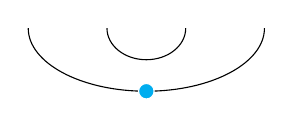
\begin{tikzpicture}[scale=1]
\dprimebox{0};
\draw (2,0)  arc (-180:0:0.5 and 0.4) ;
\draw (1,0)  arc (-180:0:1.5 and 0.8) ;
\draw[fill=cyan, draw=white]{(2.5,-0.8) circle (2.8pt)};
\end{tikzpicture},
\end{tabular}
\end{center}
then 
\begin{center}
$h_1\circ h_2=$
\begin{tabular}[c]{l}
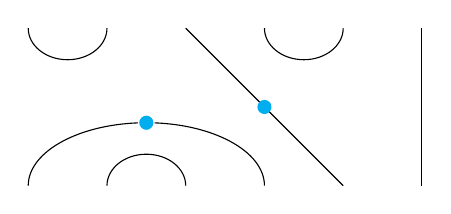
\begin{tikzpicture}[scale=1]
\sixbox{0};
\draw (1,0)  arc (-180:0:0.5 and 0.4) ;
\draw (4,0)  arc (-180:0:0.5 and 0.4) ;
\draw (2,-2)  arc (180:0:0.5 and 0.4) ;
\draw (1,-2)  arc (180:0:1.5 and 0.8) ;
\draw (3,0) -- (5,-2)
	node[fill=cyan,  pos=0.5, shape=circle, inner sep=1.8pt, minimum size=2pt]{};
\draw[fill=cyan, draw=white]{(2.5,-1.2) circle (2.8pt)};
\draw (6,0) -- (6,-2); 
\end{tikzpicture}
\end{tabular}
\end{center}
\end{example}

%\begin{figure}[!ht]
%\centering
%
%\caption{Reconstitution of two half-diagrams.}
%%$\overline{d}\circ \underline{d}$.}
%\label{IIdiag}
%\end{figure} 


We define $h$ to be a sub-half-diagram of $h'$, as shown in Figure~\ref{subhalf}, if all non-propagating edges of $h'$ are non-propagating edges of $h$. In this case, we write $h\leq h'$.

\begin{figure}[!ht]
\centering
\begin{tabular}[c]{l}
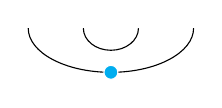
\begin{tikzpicture}[scale=0.7]
\dprimebox{0};
\draw (2,0)  arc (-180:0:0.5 and 0.4) ;
\draw (1,0)  arc (-180:0:1.5 and 0.8) ;
\draw[fill=cyan, draw=white]{(2.5,-0.8) circle (3.6pt)};
\end{tikzpicture}
\end{tabular}
$\leq$
\begin{tabular}[c]{l}

\begin{tikzpicture}[scale=0.7]
\dprimebox{0};
\draw (2,0)  arc (-180:0:0.5 and 0.4) ;
\draw (1,0)  arc (-180:0:1.5 and 0.8) ;
\draw[fill=cyan, draw=white]{(2.5,-0.8) circle (3.6pt)};
\draw (5,0) arc (-180:0:0.5 and 0.4);
\end{tikzpicture}
\end{tabular}
\caption{Example of a subhalf-diagram.}\label{subhalf}
\end{figure}  
 
The following definition of cellular algebra comes from \cite{Graham1996a}.

\begin{definition}
Let $R$ be a commutative ring with identity. A \emph{cellular algebra} over $R$ is an associative unital algebra, $A$, together with a cell datum $(\Lambda,M,C,*)$ where
\begin{enumerate}
\item $\Lambda$ is a poset. For each $\lambda\in\Lambda,M(\lambda)$ is a finite set such that 
\[
C:\coprod_{\lambda\in\Lambda}(M(\lambda)\times M(\lambda))\rightarrow A
\]
is injective with image equal to an $R$-basis of $A$.
\item If $\lambda\in\Lambda$ and $S,T\in M(\lambda)$, we write $C(S,T)=C_{S,T}^{\lambda}\in A$. Then $*$ is an $R$-linear involutory anti-automorphism of $A$ such that $(C_{S,T}^{\lambda})^*=C_{T,S}^{\lambda}$.
\item If $\lambda\in\Lambda$ and $S,T\in M(\lambda)$, then for all $a\in A$ we have
\[
aC_{S,T}^{\lambda}\equiv \sum_{S'\in M(\lambda)}r_a(S',S)C_{S',T}^{\lambda}\mod A(<\lambda),
\]
where $r_a(S',S)\in R$ is independent of $T$ and $A(<\lambda)$ is the $R$-submodule of $A$ generated by the set 
\[
\{C_{S'',T''}^{\mu}:\mu <\lambda,S''\in M(\mu),T''\in M(\mu)\}.
\]
\end{enumerate}
\end{definition}

\begin{example}
Let $S_{n}$ be the symmetric group on $n$ letters. Then the group algebra $\Z S_n$ is cellular over $\Z$. In this case, the poset $\Lambda$ is the set of partitions of $n$, ordered by dominance (meaning that if $\lambda\trianglerighteq\mu$, then $\lambda\leq\mu$). The set $M(\lambda)$ is the set of standard tableaux of shape $\lambda$, namely the ways of writing the numbers $1,2,\ldots,n$ once each into a Young diagram of shape $\lambda$ such that the entries increase along rows and down columns. The element $C^{\lambda}_{S,T}$ is the Kazhdan--Lusztig basis element $C'_w$ such that $w\in S_n$ corresponds via the Robinson--Schensted correspondence to the ordered pair of standard tableaux $(S,T)$. The map $*$ sends $C'_w$ to $C'_{w^{-1}}$. For details on standard tableaux, Young diagrams, and the Robinson--Schensted correspondence we refer the reader to \cite[Chapter 2]{Sagan2001}.
\end{example}

The Hecke algebra $\H(A_n)$ was shown to be cellular by Graham and Lehrer in \cite[Example 1.2]{Graham1996a}, and the underlying idea was already implicit in \cite{Kazhdan1979}. The example of the symmetric group above is obtained simply by specializing $q$ to 1, as was observed by Graham and Lehrer in their treatment of the Brauer algebra \cite{Graham1996a}. 

We will now construct the cell datum $(\Lambda, M, C, *)$ for $\LFD(D_n)$. Let $\Lambda$ be the set of symbols $\{1,3,5,\ldots,n\}$ when $n$ is odd and $\{0^{+},0^{-},2,4,\ldots,n\}$ when $n$ is even. We put a partial order $<$ on these symbols by declaring that $i<j$ if $\left|i\right|<\left|j\right|$, where $\left|i\right|=i$ if $i$ is a natural number, and $\left|0^{+}\right|=\left|0^{-}\right|=0$. The Hasse diagrams for the posets $\Lambda$ are shown in Figure~\ref{poset}.


\begin{figure}[!ht]
\centering
\begin{subfigure}[b]{0.48\textwidth}
\centering
\begin{tikzpicture}[scale=0.7]
\node[scale=0.6, label=left:$n$] at (1,5.8) {$\bullet$};
\node[scale=0.6, label=left:$n-2$] at (1,3.8) {$\bullet$};
\node[scale=0.6, label=left:$5$] at (1,2) {$\bullet$};
\node[scale=0.6, label=left:$3$] at (1,0) {$\bullet$};
\node[scale=0.6, label=left:$1$] at (1,-2) {$\bullet$};
\draw (1,5.8)--(1,3.8);
\node at (1,3){$\vdots$};
\draw (1,2)--(1,0)--(1,-2);
\end{tikzpicture}
\caption{$n$ odd}
\end{subfigure}
\quad
\begin{subfigure}[b]{0.48\textwidth}
\begin{tikzpicture}[scale=0.7]
\node[scale=0.6, label=left:$n$] at (1,5.8) {$\bullet$};
\node[scale=0.6, label=left:$n-2$] at (1,3.8) {$\bullet$};
\node[scale=0.6, label=left:$4$] at (1,2) {$\bullet$};
\node[scale=0.6, label=left:$2$] at (1,0) {$\bullet$};
\node[scale=0.6, label=left:$0^{+}$] at (-0.5,-2) {$\bullet$};
\node[scale=0.6, label=right:$0^{-}$] at (2.5,-2) {$\bullet$};
\draw (1,5.8)--(1,3.8);
\node at (1,3){$\vdots$};
\draw (1,2)--(1,0)--(-0.5,-2);
\draw (1,0)--(2.5,-2); 
\end{tikzpicture}
\caption{$n$ even}
\end{subfigure}
\caption{Hasse diagrams for $\Lambda$.}
\label{poset}
\end{figure}


If $\lambda\in\Lambda$, the set $M(\lambda)$ has elements parametrised by the half-diagrams $h$ arising from $D$-admissible diagrams of type II with $\mathbf{p}\left(h\right)=\left|\lambda\right|$. If $\mathbf{p}(d)=0$, then the diagram $d$ has to be reconstructed from two half-diagrams with the same parity. Hence, a half-diagram $h$ with no propagating edges will have the symbol $0^{+}$ if $h$ has an even number of decorations and $0^{-}$ if $h$ has an odd number of decorations.
The anti-automorphism $*$ corresponds to top-bottom inversion of a $D$-admissible diagram of type II.
The map $C$ takes elements $h_1$ and $h_2$ from $M(\lambda)$ and produces the element $C(h_1,h_2)$ which is defined to be $h_1\circ h_2.$

Note that the identity element appears in the image of $C$.

\begin{lemma}\label{axiomthree}
Let $\lambda\in\Lambda$ and $h_1,h_2\in M(\lambda)$. If $d=h_1\circ h_2$, then for all simple diagrams $d_i$, we have
\[
d_id=\epsilon d'
\]
for some $d'$ where $\epsilon\in\{0,1,\delta\}$ and $h_2\leq\underline{d'}$.
\end{lemma}

\begin{proof}
Since the multiplication of diagrams $d_id$ preserves the non-propagating edges in the north face of $d_i$ and the south face of $d$, $\underline{d'}$ must have at least the same non-propagating edges as $h_2$. So,  $h_2\leq\underline{d'}$. 
If $h_1$ has a non-propagating edge from node $i$ to node $i+1$ decorated with $x\in\{\emptyset,\bcirc\}$ (where $\emptyset$ denotes that the edge is undecorated), then
\[
\epsilon=\begin{cases} 0, &\mbox{ if }x=\bcirc \mbox{ and }i\neq\overline{1}\\ \delta, &\mbox{ otherwise.}\end{cases}
\]
If $h_1$ does not have a non-propagating edge from node $i$ to $i+1$, then $\epsilon=1$.% and $\underline{d'}$ has an additional non-propagating edge from node $i$ to $i+1$.
\end{proof}

\begin{remark}
The multiple $\epsilon$ does not depend on $h_2$ and $\mathbf{p}(d')\leq\mathbf{p}(d)$.
\end{remark}

Let $\LFD(D_n)\left(<\lambda\right)$ be the submodule generated by diagrams with $\mathbf{p}$-values less than $|\lambda|$. Then the following lemma holds.

\begin{lemma}\label{lessnonprop}
Let $d,d'\in\LFD(D_n)$. If $\mathbf{p}(d')<\mathbf{p}(d)$, then $d'\in \LFD(D_n)\left(<\lambda\right)$, where $|\lambda|=\mathbf{p}(d)$.
\qed
\end{lemma}

%%%%%%%%%%%%%%%%

\begin{theorem}\label{loopfreecellular}
The algebra $\LFD(D_n)$ over the ring $\Z[\delta]$ has a cell datum $(\Lambda,M,C,*)$, where the sets are given as above.
\end{theorem}

\begin{proof}
The proof is largely straightforward. The only nontrivial part is the verification of axiom 3. Since $\LFD(D_n)$ is generated by the simple diagrams, it is enough to multiply $d$ by a simple diagram and hence axiom 3 follows quickly from Lemma~\ref{axiomthree} and Lemma~\ref{lessnonprop}.
% Consider the product of two basis elements $B$ and $B'$ parametrised by the respective elements $\lambda$ and $\lambda'$ of $\Lambda$. The only difficulty aries when 
\end{proof}

Since $\LFD(D_n)\cong\PFTL(D_n)$ as $\Z[\delta]$-algebras, the following corollary is immediate.

\begin{corollary}\label{pairfreecellular}
The algebra $\PFTL(D_n)$ over the ring $\Z[\delta]$ is cellular.
\qed
\end{corollary}

\section{Future work}

We have shown that $\PFTL(D_n)$ is cellular by explicitly constructing a cell datum for $\LFD(D_n)$. However, it remains to describe the corresponding cell datum for $\PFTL(D_n)$, which may or may not be enlightening.  As an application, we could utilize the structure of the algebra to quickly compute $\mu$-values (see Section~\ref{hecke}) for pairs of elements that index the basis of $\PFTL(D_n)$. 

We have shown that a quotient of $\TL(D_n)$ is cellular, but we are uncertain if $\TL(D_n)$ itself is cellular. This is likely known, but we are unable to find a reference.

Lastly, it is known that there is a connection between $\PFTL(D_n)$ and the so-called blob algebra \cite{Martin1994}. Future work could include making this connection more explicit.

%Some future work includes showing that $\PFTL(D_n)$ is well-behaved with respect to the Kazhdan--Lusztig basis and what is the corresponding cell datum for $\PFTL(D_n)$. This is likely known to the experts in the field, but does not explicitly appear in the literature. As an application, we could utilize the structure of the algebra to quickly compute $\mu$-values for pairs of elements that index the basis of $\PFTL(D_n)$. Moreover, we can show how $\PFTL(D_n)$ is connected to the blob algebra of \cite{Martin1994}. Also, if $\PFTL(D_n)$ is cellular, is $\TL(D_n)$ cellular?